\documentclass[onecolumn,12pt]{article}

\usepackage[utf8]{inputenc}
\usepackage[T1]{fontenc}
\usepackage{polski}

\setlength{\voffset}{-0.55in}
\setlength{\headsep}{3pt}

\usepackage{hyperref}
\hypersetup{
    colorlinks=false, %set true if you want colored link
    linktoc=all,     %set to all if you want both sections and subsections linked
}

\usepackage[polish]{babel}
\usepackage{algorithm,algorithmic,lipsum}
\usepackage[utf8]{inputenc}
\usepackage{url}
\usepackage{anyfontsize}
\usepackage{multirow}
\usepackage{subfigure}
\usepackage{tabularx}
\usepackage{ragged2e}
\usepackage{booktabs}
\usepackage{multirow}
\usepackage{grffile}
\usepackage{indentfirst}
\usepackage{caption}
\usepackage{listings}
\usepackage{lipsum}
\usepackage{enumitem}
%\usepackage{xcolor}
%\usepackage{hyperref}
\usepackage{catchfilebetweentags}
\usepackage[smartEllipses]{markdown}
\usepackage[ruled,linesnumbered,lined]{algorithm2e}
\usepackage[bookmarks=false]{hyperref}
\usepackage{mathtools}
\DeclarePairedDelimiter\ceil{\lceil}{\rceil}
\DeclarePairedDelimiter\floor{\lfloor}{\rfloor}

\hypersetup{colorlinks,
    linkcolor=blue,
    citecolor=blue,
    urlcolor=blue}

\usepackage[svgnames]{xcolor}
\usepackage{inconsolata}
\usepackage{fontawesome}

\usepackage{csquotes}
\DeclareQuoteStyle[quotes]{polish}
    {\quotedblbase}
    {\textquotedblright}
    [0.05em]
    {\quotesinglbase}
    {\fixligatures\textquoteright}
\DeclareQuoteAlias[quotes]{polish}{polish}

\usepackage[nottoc]{tocbibind}


\usepackage[
style=numeric,
sorting=nyt,
isbn=false,
doi=true,
url=true,
backref=false,
backrefstyle=none,
maxnames=10,
giveninits=true,
abbreviate=true,
defernumbers=false,
backend=biber]{biblatex}

\lstset{
        %language=Python,  %%  PHP,  C,  Java,  etc.
        basicstyle=\ttfamily\footnotesize,
        backgroundcolor=\color{gray!5},
        commentstyle=\it\color{Green},
        keywordstyle=\color{Red},
        stringstyle=\color{Blue},
        numberstyle=\tiny\color{Black},        
        %  morekeywords={TestKeyword},
        %  mathescape=true,
        escapeinside=`',
        frame=single,  %shadowbox,  
        tabsize=2,
        rulecolor=\color{black!30},
        title=\lstname,
        breaklines=true,
        breakatwhitespace=true,
        framextopmargin=2pt,
        framexbottommargin=2pt,
        extendedchars=false,
        captionpos=b,
        abovecaptionskip=5pt,
        keepspaces=true,                        
        numbers=left,                                        
        numbersep=5pt,                                    
        showspaces=false,                                
        showstringspaces=false,
        showtabs=false,
        tabsize=2
    }

\definecolor{graytext}{gray}{0.6}

\lstdefinestyle{PostgreSQL}{
    literate={ą}{{\k a}}1
    		 {Ą}{{\k A}}1
             {ż}{{\. z}}1
             {Ż}{{\. Z}}1
             {ź}{{\' z}}1
             {Ź}{{\' Z}}1
             {ć}{{\' c}}1
             {Ć}{{\' C}}1
             {ę}{{\k e}}1
             {Ę}{{\k E}}1
             {ó}{{\' o}}1
             {Ó}{{\' O}}1
             {ń}{{\' n}}1
             {Ń}{{\' N}}1
             {ś}{{\' s}}1
             {Ś}{{\' S}}1
             {ł}{{\l}}1
             {Ł}{{\L}}1,
    keywordstyle=\textbf,
}

\SetAlgorithmName{\LangAlgorithm}{\LangAlgorithmRef}{\LangListOfAlgorithms}
\newcommand{\listofalgorithmes}{\tocfile{\listalgorithmcfname}{loa}}

\renewcommand{\lstlistingname}{\LangListing}
\renewcommand\lstlistlistingname{\LangListOfListings}

\renewcommand{\lstlistoflistings}{\begingroup
\tocfile{\lstlistlistingname}{lol}
\endgroup}

\begin{document}
% ----------Strona tytułowa------------
\title{Symulacje procesów ciągłych i algorytmy adaptacyjne\\
Projekt –Symulacja wydobywania ropy}
\author{Magdalena Królikowska, Gabriela Piwar, Sławomir Tenerowicz}
\date{\today}
\maketitle

% ----------Spis treści------------
\tableofcontents
\thispagestyle{empty}

% ----------Raport------------
\section{Wprowadzenie}

 Wydobywanie ropy naftowej to kluczowy proces dla światowej gospodarki, stanowiący podstawę dla wielu gałęzi przemysłu. Jest to nie tylko jedno z głównych źródeł energii, ale także surowiec niezbędny do produkcji wielu produktów chemicznych i petrochemicznych. Z uwagi na strategiczne znaczenie ropy naftowej, optymalizacja procesów wydobywczych oraz zrozumienie mechanizmów zachodzących podczas eksploatacji złoża są niezwykle istotne.

Symulacje komputerowe stanowią narzędzie, które umożliwia lepsze zrozumienie i optymalizację procesów wydobywczych. Poprzez modelowanie różnych scenariuszy oraz warunków geologicznych, symulacje mogą wspomóc podejmowanie decyzji w zakresie projektowania i eksploatacji złóż ropy naftowej.

\section{Cel projektu}

Celem projektu było stworzenie symulacji wydobywania ropy naftowej poprzez
szczelinowane hydrauliczne. W tym celu zmodyfikowaliśmy załączone pliki oil2d.hpp i oil2d.cpp, które poźniej posłużyły do uruchomienia skryptów symulacji
w solverze IGA-ADS.
        
\section{Opis rozwiązania}

W tej cześci omówiono kroki podjęte w celu modyfikacji kodu symulacyjnego. Należały do nich:  
\begin{enumerate}
    \item zaprojektowanie mapy warstw geologicznych 
    \item zaprojektowanie i umieszczenie na mapie pomp ssących i pompujących 
\end{enumerate}


\subsection{Modyfikacja mapy geologicznej.}

Wczytano zadaną mapę warstw geologicznych i przekonwertowano ją w taki sposób, aby zawierała wartości z przedziału [0,1]. Wartości mapy zapisano do pliku csv, który następnie posłużył do inicjalizacji macierzy permeability\_matrix.

\begin{figure}[H]
    \centering
    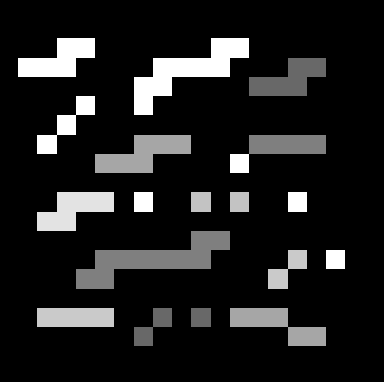
\includegraphics[width=0.9\textwidth]{init_matrix.png}
    \caption{Mapa warstw geologicznych z wartościami w przedziale [0,1]}
    \label{fig:example}
\end{figure}

Zmodyfikowano funkcję permeability() tak, by korzystała z macierzy permeability\_matrix.
\begin{figure}[H]
    \centering
    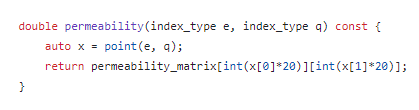
\includegraphics[width=0.9\textwidth]{permeability.png}
    \caption{Modyfikacja funkcji permeability()}
    \label{fig:example}
\end{figure}

Zmodyfikowano funkcję fill\_permeability\_map() tak, by korzystała z macierzy permeability\_matrix.
\begin{figure}[H]
    \centering
    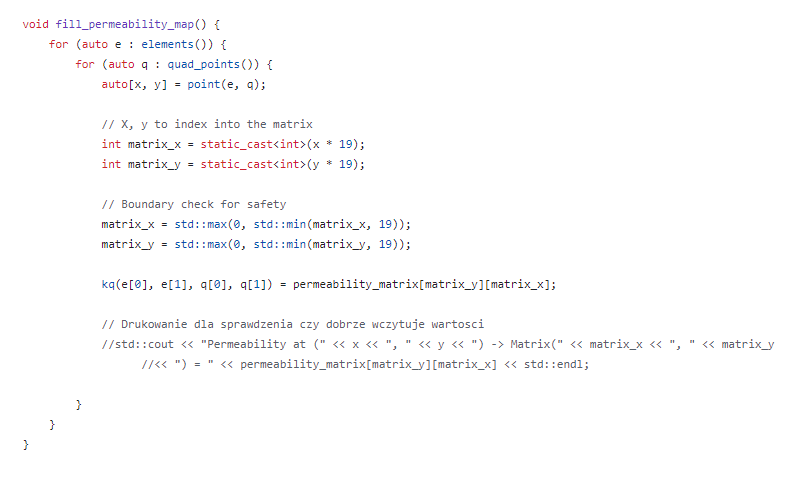
\includegraphics[width=0.9\textwidth]{fill_permeability_map.png}
    \caption{Modyfikacja funkcji fill\_permeability\_map()}
    \label{fig:example}
\end{figure}

\subsection{Modyfikacja ustawienia pomp.}
 
\begin{figure}[H]
    \centering
    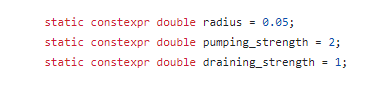
\includegraphics[width=0.9\textwidth]{pumps_params.png}
    \caption{Modyfikacja parametrów pomp.}
    \label{fig:example}
\end{figure}
\section{Wyniki}

Rysunki przedstawiają konkretne kroki czasowe symulacji.

\begin{figure}[H]
    \centering
    \subfloat{{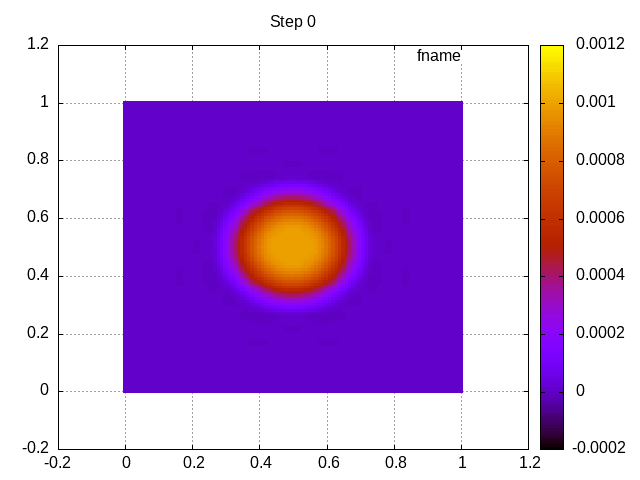
\includegraphics[width=6cm]{0.png} }}%
    \qquad
    \subfloat{{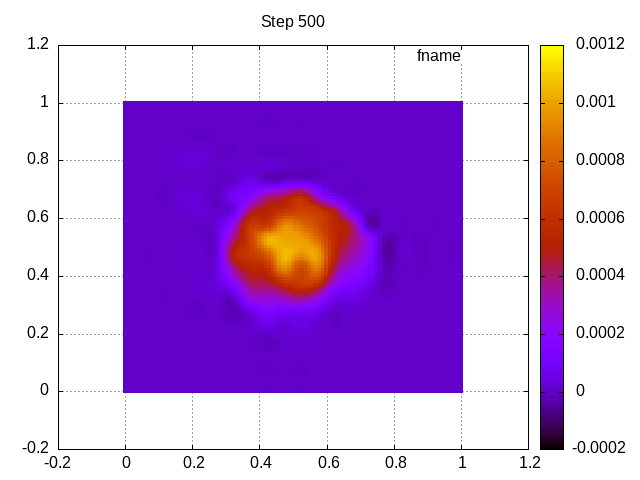
\includegraphics[width=6cm]{500.png} }}%
    \qquad
    \subfloat{{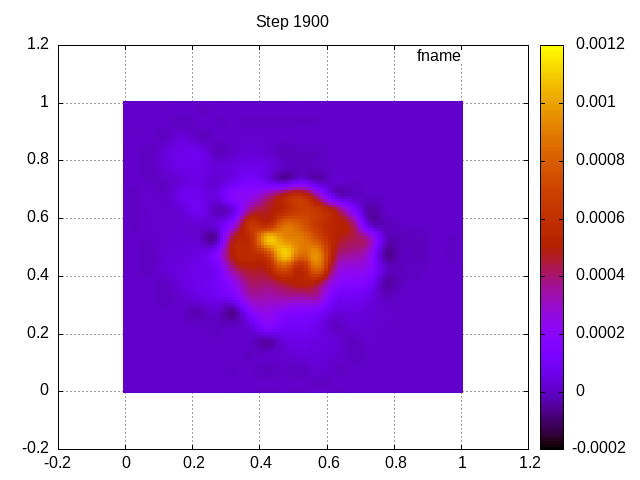
\includegraphics[width=6cm]{1900.png} }}%
    \qquad
    \subfloat{{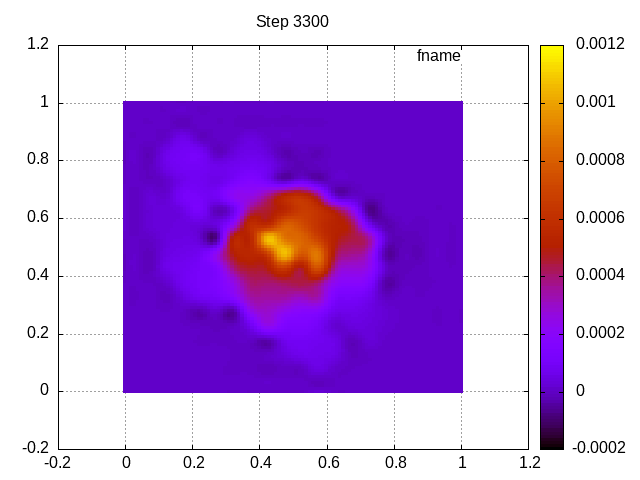
\includegraphics[width=6cm]{3300.png} }}%
    \qquad
    \subfloat{{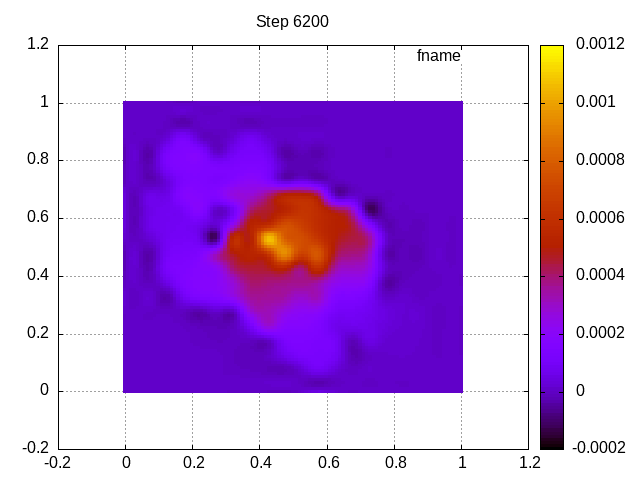
\includegraphics[width=6cm]{6200.png} }}%
    \qquad
    \subfloat{{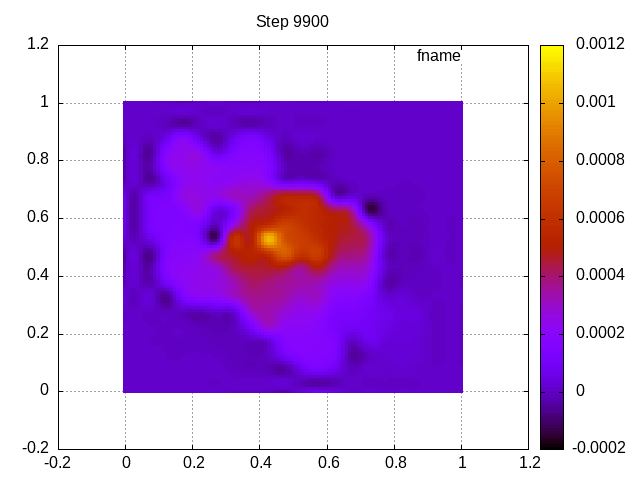
\includegraphics[width=6cm]{9900.png} }}%
    \caption{Kolejne klatki z otrzymanej symulacji.}%
\end{figure}

\section{Podsumowanie}
udalo sie? 


\begin{thebibliography}{9}

\end{thebibliography}

\end{document}
